\section{Theorie}
\label{sec:Theorie}

\subsection{Schubmodul G}
Das Schubmodul oder auch Torsionsmodul G bezeichnet die Gestaltselastizität eines Körpers.\\
Wenn ein Körper um einen Winkel \(\alpha\) verbogen wird, so ensteht eine Schubspannung \(\tau\).
Die Beziehung zwischen beiden Größen wird mit G beschrieben:
\begin{equation}
    \tau = G\alpha
    \label{eq:formel1}
\end{equation}
Um einen zylindrischen Draht zu verdrehen, braucht es zwei tangentiale entgegengesetzte Kräfte \(\vec{K}\) und \(-\vec{K}\), die das Drehmoment M des Drahtes mit Radius r mit
\begin{equation}
    dM = r \ dK
    \label{eq:formel2}
\end{equation}
beschreiben. 
Gleichzeitig kann die Schubspannung \(\tau\) durch
\begin{equation}
    \tau = \frac{dK}{dF}
    \label{eq:formel3}
\end{equation}
ausgedrückt werden, wobei dF für eine Flächeneinheit steht.\\
Aus \autoref{eq:formel1}, \autoref{eq:formel2} und \autoref{eq:formel3} ergibt sich die Beziehung:
\begin{equation}
    dM = r \ G\alpha \ dF
    \label{eq:formel4}
\end{equation}
\newpage
Die \autoref{fig:skizze1} zeigt einen Zusammenhang aller nötigen Größen für die weitere Rechnung.\\
\begin{figure}
    \centering
    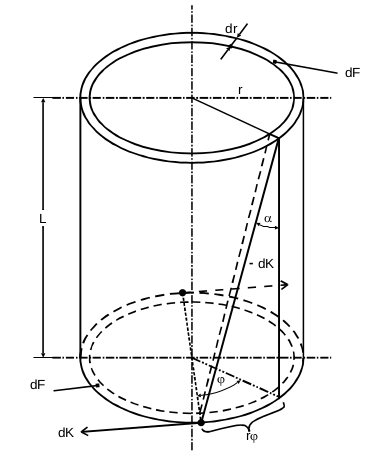
\includegraphics[scale=0.5]{content/Bilder/Skizze1.png}
    \caption{Skizze zur Darstellung des Zusammenhangs der Rechnungsgrößen an einem zylindrischen Draht.}
    \label{fig:skizze1}
\end{figure}
Wie zu erkennen ist, beschreibt der Torsionswinkel \(\phi\) einen Weg \(r_{\phi}\) entlang des verdrehten Außenrands.
\begin{equation}
    \alpha = \frac{r_{\phi}}{L}
    \label{eq:formel5}
\end{equation}
Der Flächeninhalt des Kreisringes in \autoref{fig:skizze1} ergibt sich aus:
\begin{equation}
    dF = 2\pi \ r \ dr
    \label{eq:formel6}
\end{equation}
Zusammen ergeben (4), (5) und (6) die Gleichung für das Trägheitsmoment in differentieller Form:
\begin{equation}
    dM = 2\pi \ \frac{G}{L} \ \phi r^3 \ dr
    \label{eq:formel7}
\end{equation}
Über den Proberadius R integriert, lautet die Formel für M dann:
\begin{equation}
    M = \frac{\pi}{2}G\frac{R^4}{L}\phi
    \label{eq:formel8}
\end{equation}
Die sogenannte Richtgröße des Zylinders lautet hierbei:
\begin{equation}
    D := \frac{\pi G R^4}{2L}
    \label{eq:formel9}
\end{equation}
\\
Die resultierende Bewegungsgleichung des Systems setzt sich dann aus \autoref{eq:formel8} und der \textit{Trägheit der rotierenden Masse} zusammen:
\begin{equation}
    D\phi \ +\ \theta\frac{d^2\phi}{dt^2} = 0
    \label{eq:formel12}
\end{equation}
Die Lösung dazu lautet:
\begin{equation}
    \phi(t) = \phi_0\cos\frac{2\pi}{T}t \quad\textrm{mit}\quad T = 2\pi\sqrt{\frac{\theta}{D}}
    \label{eq:formel10}
\end{equation}
\\
\
\\
Da an dem Draht eine Kugel hängt, lässt sich der Winkel $\theta_{Kugel}$ durch
\begin{equation}
    \theta_{Kugel} = \frac{2}{5}m_KR_K^2
    \label{eq:formel11}
\end{equation}
beschreiben, wobei $m_K$ die Kugelmasse ist und $R_K$ der Radius.\\
Aus \autoref{eq:formel9}, \autoref{eq:formel10} und \autoref{eq:formel11} setzt sich G zusammen:
\begin{equation}
    G = \frac{16}{5}\ \pi\ \frac{m_KR_K^2L}{T^2R^4}
    \label{eq:formelG}
\end{equation}
\newpage
\subsection{Poissonsche Querkontraktionszahl \texorpdfstring{$\mu$}{mu} \& Kompressionsmodul Q}
Sowohl $\mu$ als auch Q hängen von G und dem Elastizitätsmodul E ab.
Ihre Beziehung lässt sich durch
\begin{equation}
    E = 2G(\mu\ +\ 1)\\
    \
    \textrm{und}\\
    \
    E = 3(1\ -\ 2\mu)Q
    \label{eq:formelE}
\end{equation}
darstellen.\\
Die Querkontraktionszahl $\mu$ ist eine elastische Konstante, die angibt, wie groß die Längenänderung eines gedehnten Körpers ist.
Das Kompressionsmodul Q, ebenfalls eine elastische Konstante, gibt die Volumenänderung an.\\
\subsection{Magnetisches Moment}
Um ein magnetisches Moment mittels Torsion zu berechnen, verwendet man eine ähnliche Formel wie \autoref{eq:formel12}, die m enthält.
Nach m aufgelöst, lässt es sich dann durch
\begin{equation}
    m = \frac{4\pi^2\theta}{T_B^2B}\ -\ \frac{D}{B}
    \label{eq:formel13}
\end{equation}
berechnen.
\subsection{Gauß'sche Fehlerfortpflanzung}
Die bei der Auswertung verwendeten Größen wurden gemäß der Gauß'schen Fehlerfortpflanzung berechnet.
Die Formel dafür lautet:
\begin{equation}
    \overline{v_x}=\frac{1}{N} \sum_{j=1}^N v_j
\end{equation}
für den Mittelwert der Messung, und
\begin{equation}
    u_x = \sqrt{\frac{1}{N(N-1)} \sum_{j=1}^N (v_j-\overline{v_x})^2}
\end{equation}
für die Unsicherheiten der Messwerte $v_x$.